% This LaTeX was auto-generated from MATLAB code.
% To make changes, update the MATLAB code and export to LaTeX again.


\documentclass{scrreprt}

\usepackage{geometry}
\usepackage[utf8]{inputenc}
\usepackage{blindtext}
\usepackage[T1]{fontenc}
\usepackage{lipsum}
\usepackage{hyperref}
\usepackage{enumitem}
\usepackage{graphicx}
\usepackage{float}
\usepackage{hyperref}

\hypersetup{
    colorlinks=true,
    linkcolor=blue,
    filecolor=magenta,      
    urlcolor=cyan,
}

\urlstyle{same}

\newlength\mylen
\setlength\mylen{0.5in}
\geometry{letterpaper, portrait, lmargin=1.5in, tmargin=1in}

\renewcommand*{\chapterformat}{%
  \llap{\protect\makebox[\mylen][l]{\chapappifchapterprefix{\nobreakspace}\thechapter\autodot\hfill}}%
}




\begin{document}
\begin{titlepage}

\begin{center}
       \vspace*{5cm}




       {\Huge \textbf{USER MANUAL}}\\
       \vspace{0.5cm}
       Microdroplet Impact Video Processing Applet\\
       v1.0\\
	Release Date: April 21, 2021\\
       \vspace{1.5cm}


       \vfill
            
	Rosemary Barrass\\Zachariah Weber\\Andrew Tunison\\Nikita Kurilenko\\
	\vspace{0.5cm}
	Developed under the guidance of\\Dr. Hua Tan\\Assistant Professor of Mechanical Engineering\\Washington State University Vancouver\\
	\vspace{1.5cm}      
 	
\includegraphics[width=0.4\textwidth]{university}\\
	Engineering and Computer Science Department\\
       Washington State University Vancouver\\
       
 
            
\end{center}

\end{titlepage}


\tableofcontents
\newpage

\chapter{Introduction}


\section{Purpose}
The purpose of this document is to describe the operating steps, description theory, and fault isolation procedures of the microdroplet impact analysis software. 


\section{Document Conventions}
In this document the variables and functions will be called exactly as they are in the program code. Function inputs and outputs of the same name across multiple functions refer to the same variable unless otherwise indicated. 

\section{Intended Audience}
MATLAB Microdroplet Impact Analysis Application is designed for students, professors, professionals, and anyone interested in analyzing microdroplet impacts. This application was initially designed for Interfacial Fluid Dynamics Lab at Washington State University Vancouver. However, this is an open-source program and can be used by anyone. 

\section{Product Scope}
This applet is to be used for automated processing of microfluid droplet videos. This applet takes an input of .avi video files and provides a table of parameters for instantaneous primary droplet velocity, primary droplet spread radius, satellite droplet velocity, number of satellite droplets per frame, jet velocity, jet diameter, jet tip position, primary droplet contact angle, maximum primary droplet spread radius, and maximum primary droplet velocity. This data is intended for use in aiding research in microfluid behavior. This applet is not intended to replace logical reasoning, so data taken from this applet should be checked before use in academic research in case errors have occurred in processing.























\chapter{Overall Description}


\section{Product Perspective}
This applet reduces the need for extensive image processing training and coding for researchers, as it provides much of the basic parameters that are necessary for microfluid droplet analysis. However, this applet is a living code that needs continuous updates to be compatible with a wide range of droplet videos. At its current iteration, this applet can be used on droplets with high contrast against their environment that move vertically from the perspective of the camera.

\section{Product Functions}
The applet can be used to output:
\begin{itemize}
\item Basic microdroplet parameters, such as:
\begin{itemize}
\item primary and satellite droplet velocity
\item primary droplet spread radius
\item primary droplet contact angle
\item jet speed
\item jet diameter
\item jet tip position
\item number of satellite droplets
\end{itemize}

\item Individual processed frames with either droplet outlines or contact angle lines.

\end{itemize}

\section{User Classes and Characteristics}
The user classes for this applet include undergraduate, graduate, and postgraduate researchers as well as university instructors and researchers. Undergraduate researchers are likely to be using laptops or other computers with limited memory resources. These users will also be performing introductory levels of analysis of microfluid droplet behavior. Graduate, postgraduate, and university researchers are likely to have access to high performing computing, such as that provided by computing clusters. These users are likely to be performing higher level analysis of microfluid droplet behavior and are more likely to be able to spot processing errors if they arise. For all user classes, this applet provides many of the key parameters necessary for conducting microfluid droplet analysis without the need to learn image processing algorithms or extensive MATLAB coding tools.

\section{Operating Environment}
This applet was created in MATLAB, which has been tested on Mac, Windows, and Ubuntu operating systems. This applet was created and tested using Windows.

\section{Design and Implementation Constraints}
This applet is constrained to use on microfluid droplet videos in the .avi format. Future iterations may be implemented for use with a wider range of video formats. The applet is also unable to process droplets that are clear or provide little contrast to the background. Input videos must be converted to grayscale prior to use in the applet. The user is expected to provide high quality input videos for optimal processing.

\section{User Documentation}
Any user of this applet is the target audience of this user documentation. For users that may be altering the code of the GUI or image processing functions, additional documentation found on the MathWorks website is suggested as a supplemental resource.

\section{Assumptions and Dependencies}
It is required that the user of the applet has the MATLAB Image Processing Toolbox installed. It is assumed that all users of this applet have at least a basic understanding of microfluid analysis and an ability to understand MATLAB error messages. 

\chapter{GUI User Guide}
In this chapter, a step-by-step guide for the use of the GUI is provided, with images.

\section{Installation}

\begin{enumerate}[label = Step \arabic*.]

\item Double left-click on GUI\_Design.mlappinstall. \\
\item Left-click on "Install" on pop-up window.
\begin{figure}[H]
\centering
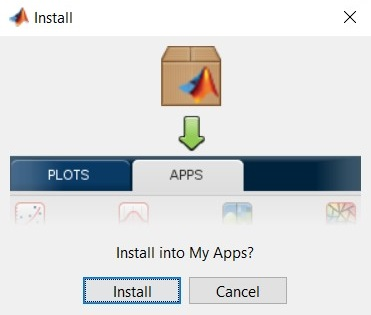
\includegraphics[width=0.5\textwidth]{InstallIntoMyApps.jpg}
\label{fig:installpopup}
\end{figure}
\end{enumerate}

\section{Opening the Applet}

\begin{enumerate}[label = Step \arabic*.]

\item Open MATLAB. \\
\item Left-click on the "APPS" tab in the top left corner of the MATLAB environment
\begin{figure}[H]
\centering
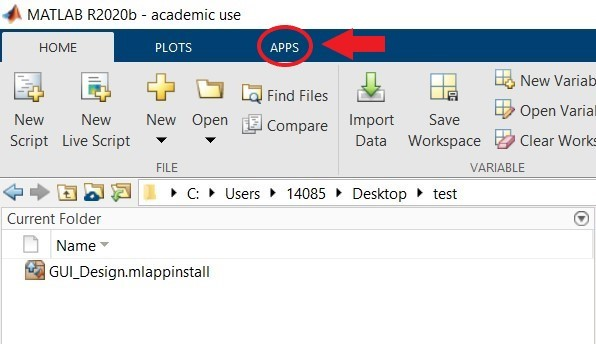
\includegraphics[width=0.5\textwidth]{FindingApps.jpg}
\label{fig:appstablocation}
\end{figure} 

\item Left-click on the dropdown menu in the APPS bar.
\begin{figure}[H]
\centering
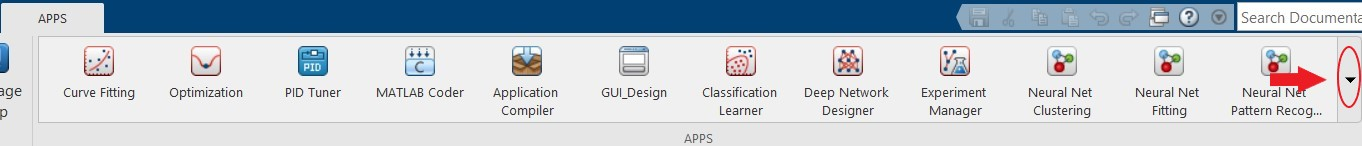
\includegraphics[width=\textwidth]{APPSDropDown.jpg}
\label{fig:appsdropdown}
\end{figure}

\item From the dropdown menu, left-click GUI\_Design from the "MY APPS" section.
\begin{figure}[H]
\centering
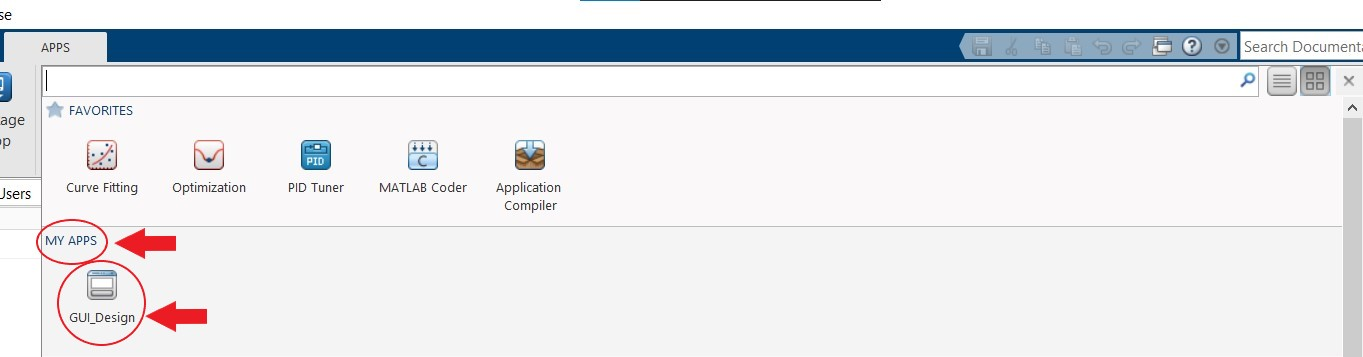
\includegraphics[width=0.5\textwidth]{MyAppsSection.jpg}
\label{fig:myappssection}
\end{figure}

\end{enumerate}

\section{Using the Applet}

\subsection{Uploading a Video}

\begin{enumerate}[label = Step \arabic*.]

\item Left-click on the "Upload Video" button. 
\begin{figure}[H]
\centering
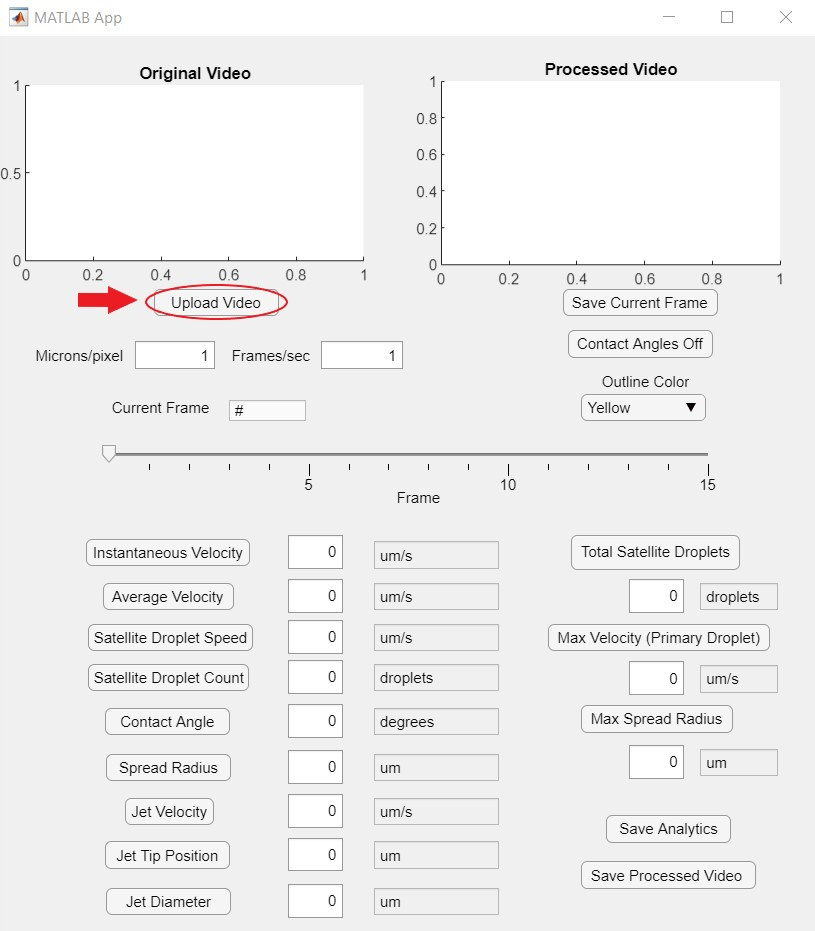
\includegraphics[width=0.5\textwidth]{appletbeforeupload.jpg}
\label{fig:uploadvideobutton}
\end{figure}

\item Select the video you would like to upload from the File Explorer window. Select "Open" to open that video file in the applet. The applet will open a secondary window for floor selection. You can either use the interactive floor finding or input the floor height in pixels and the floor angle. \\

\end{enumerate}

\subsubsection{Interactive Floor Finding}
\begin{enumerate}[label = Step \arabic*.]

\item Left-click the "Start Interactive Floor Find" button.
\begin{figure}[H]
\centering
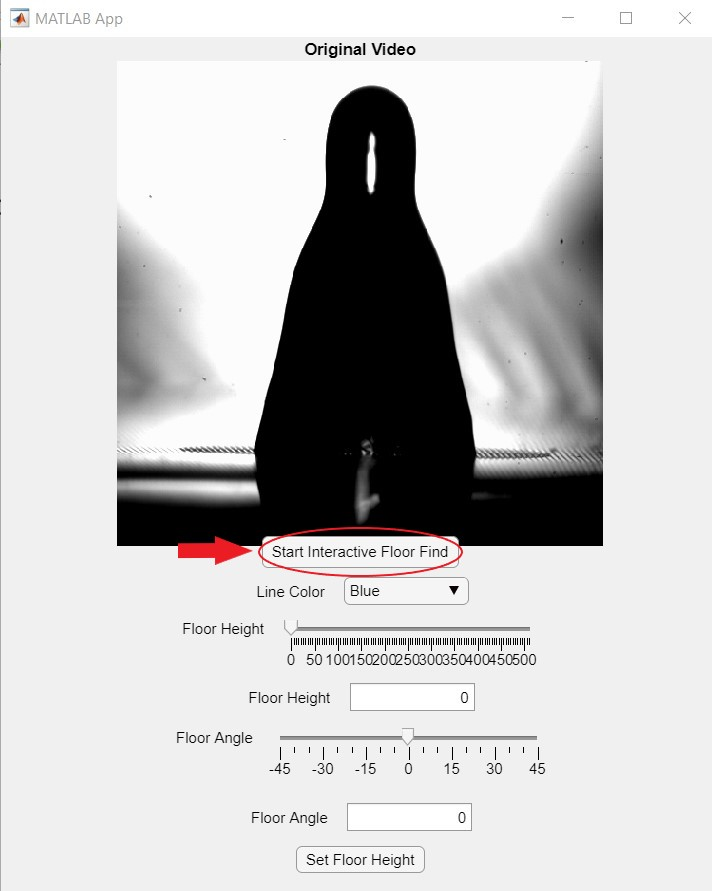
\includegraphics[width=0.5\textwidth]{SecondaryAppletFloorFindButton.jpg}
\label{fig:interactivefloorfindbutton}
\end{figure}

\item An instructional message will appear, informing the user that they can now draw a line at the floor on the video frame. Press the "OK" button to proceed with the interactive floor finding.
\begin{figure}[H]
\centering
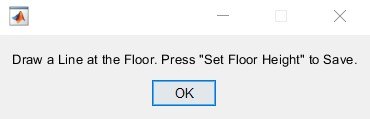
\includegraphics[width=0.5\textwidth]{DrawALineMsg.jpg}
\label{fig:drawalinemsg}
\end{figure}

\item Left-click and drag on the image to draw a line for the floor. To move this line, left-click and drag either blue dot at the ends of the line. Use the "Zoom-In" feature in the upper right-hand corner of the image to get a better look at where the floor line is located on the image. Continue manipulating the line by moving the blue dots until the interactive floor line matches the line of the floor in the original image. Press "Set Floor Height" Button once the interactive line is aligned.

\begin{figure}[H]
\centering
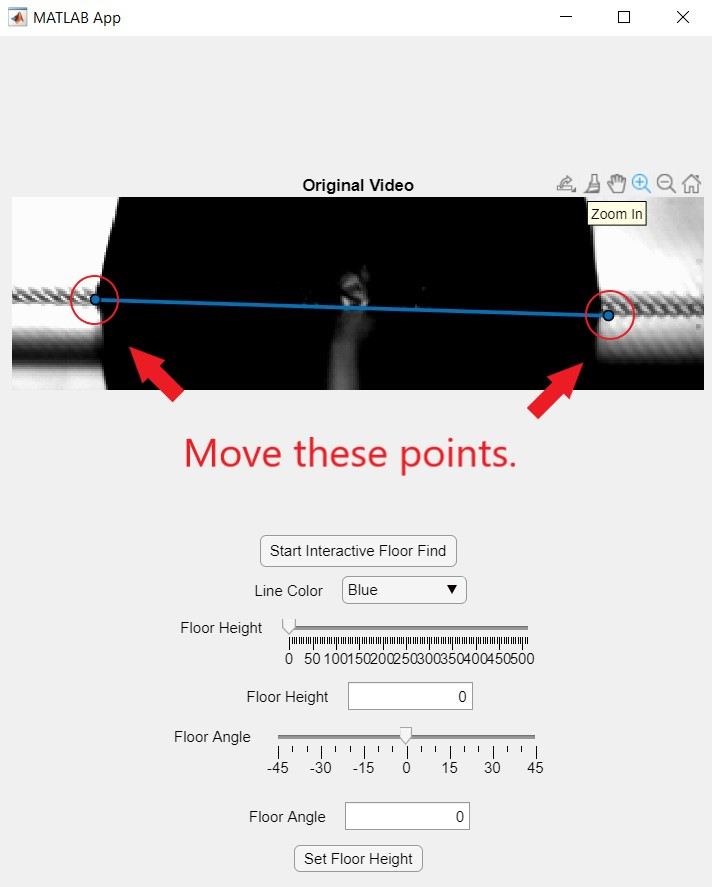
\includegraphics[width=0.5\textwidth]{InteractiveFloorLine.jpg}
\label{fig:interactiveline}
\end{figure}

\subsubsection{Manual Floor Height and Angle Entry}
During the manual floor height and angle entry process, if the line is difficult to see, the user can select a different line option from the "Line Color" dropdown menu. This feature is ONLY available for the line printed by manual floor height and angle entry.


\item Move the slider next to "Floor Height" or manually enter floor height value into the textbox below to set a floor height. Note: "Floor Height" is measured in pixels, counting the number of pixels from the top of the image to the centermost pixel of the floor line.
\begin{figure}[H]
\centering
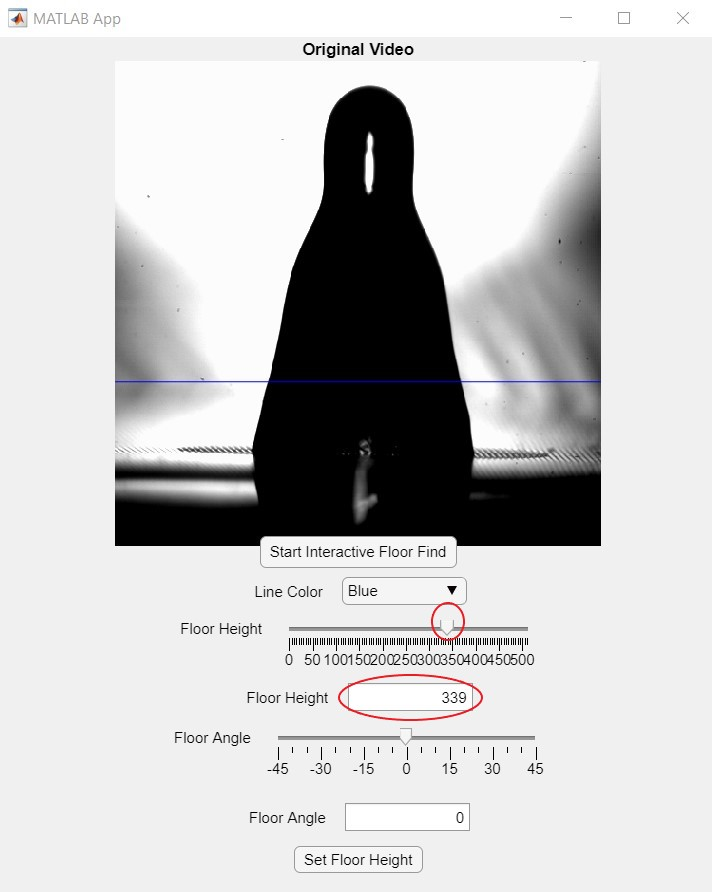
\includegraphics[width=0.5\textwidth]{ManualFloorHeight.jpg}
\label{fig:manualfloorheightslct}
\end{figure}

\item Move the slider next to "Floor Angle" or manually enter floor angle value into the textbox below to set a floor angle. 
\begin{figure}[H]
\centering
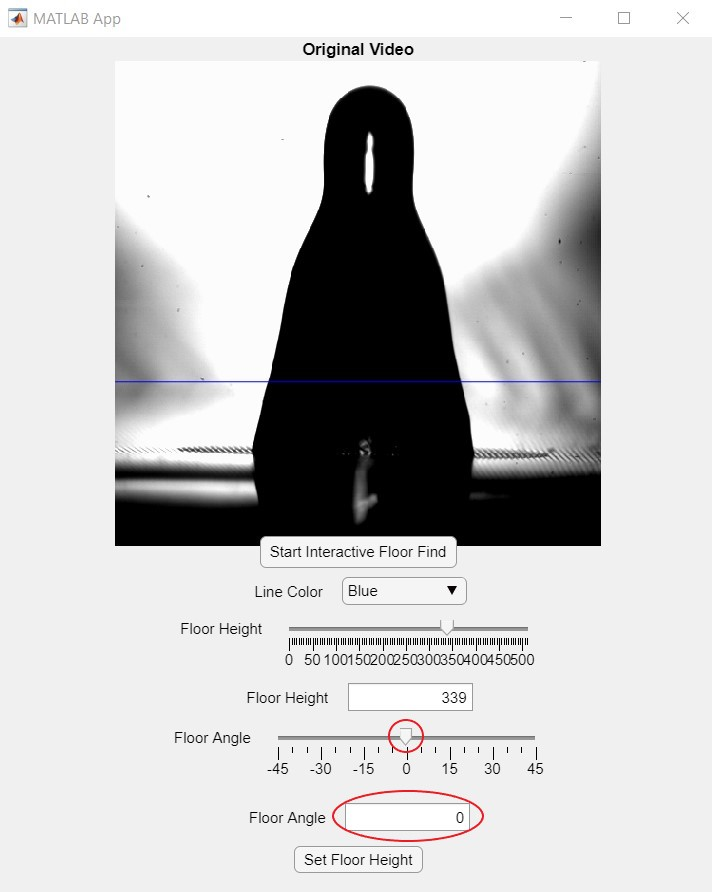
\includegraphics[width=0.5\textwidth]{ManualFloorAngle.jpg}
\label{fig:manualfloorangleslct}
\end{figure}

\item Once both floor height and floor angle are at the correct values, left-click the "Set Floor Height" button to input the floor values.

\item Once the floor height and angle has been set, the applet will process the entire video, then display the processed video. Please note, this process takes a lot of computation and will take time, especially on computers with limited processing power. 
\begin{figure}[H]
\centering
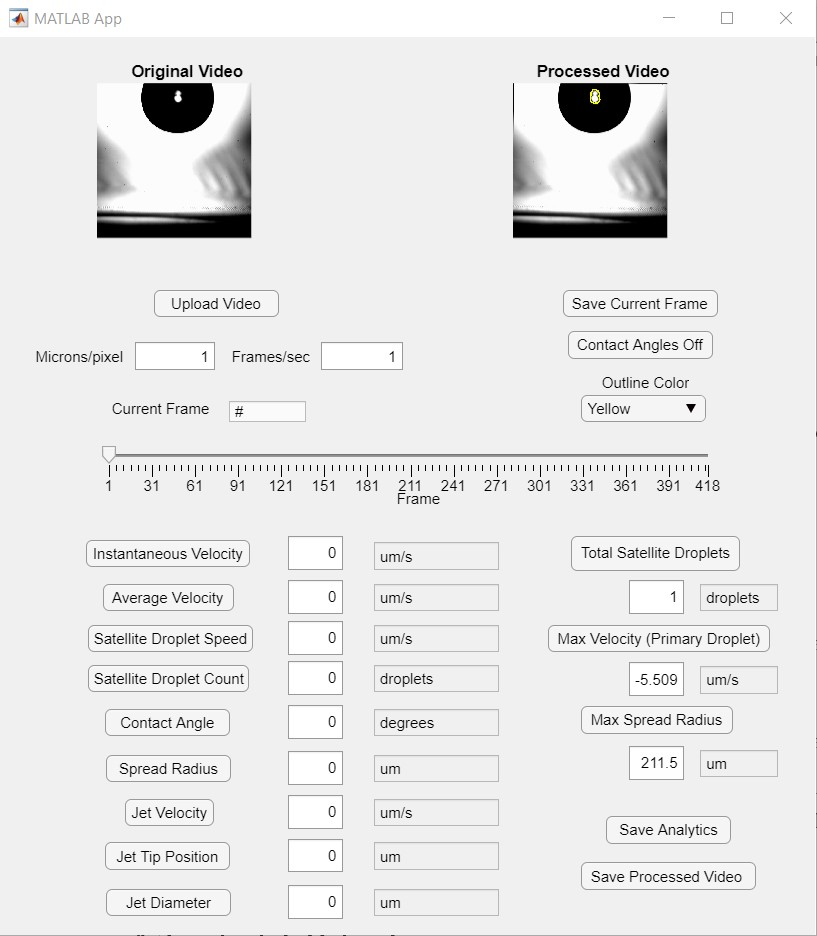
\includegraphics[width=0.5\textwidth]{FirstProcessedVideoImage.jpg}
\label{fig:rightafterfloorfind}
\end{figure}
\end{enumerate}

\subsection{Applet Features}

The following section describes the function and interactivity of each feature, listed in order as marked in the figure below.

\begin{figure}[H]
\centering
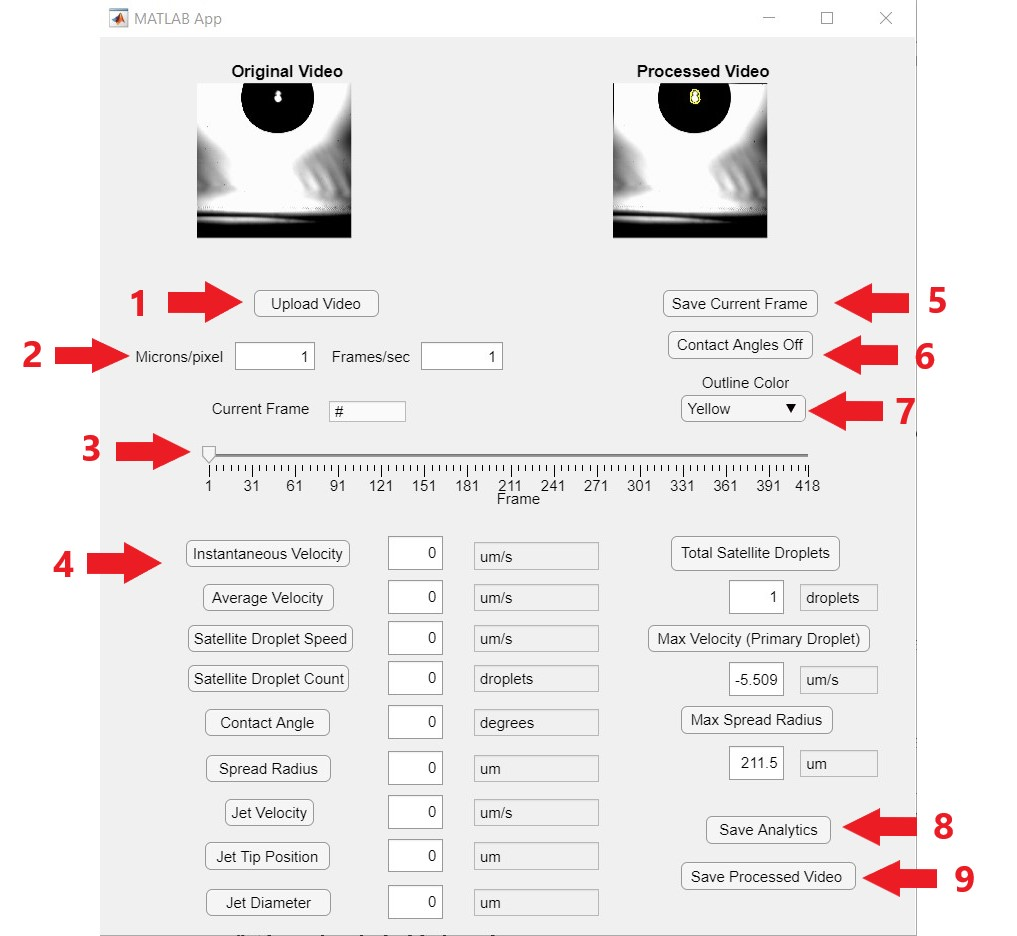
\includegraphics[width=0.5\textwidth]{AppletFeatures.jpg}
\label{fig:appletfeatures}
\end{figure}

\begin{enumerate}[label = \textbf{Feature \arabic*.}]

\item Upload Video Button. \\

\textbf{Function:} The upload video button allows the user to select a video file from the file explorer window to upload to the applet for processing. \\
\textbf{Interactivity:} The user can press the button to activate the button-down callback.

\item Micron/pixel and Frame/sec text boxes. \\

\textbf{Function:} These text boxes are used to change the micron/pixel ratio and frame/second ratio for the parameters found by the applet. The applet automatically converts all values using the user's input.\\
\textbf{Interactivity:} The user can type a decimal value into the text boxes to activate the value changed callback.

\item Frame Slider. \\

\textbf{Function:} The frame slider is used to change the current frame displayed in the original and processed video image boxes. This also changes the displays of all of the parameter text boxes to show the value of each parameter at the newly selected frame. The frames and values change in real-time as the user interacts with the slider.\\
\textbf{Interactivity:} The user can right-click on any point along the line to activate the value changed callback. The user can right-click and drag the indicator along the line to activate the value changing callback.

\item Parameter Text Boxes. \\

\textbf{Function:} The parameter text boxes display the various calculated parameters that the applet obtains from the video. Some values displayed are calculated per frame, while others are calculated for the entire video (i.e., max spread radius is the maximum for the whole video).\\
\textbf{Interactivity:} The user cannot interact directly with these text boxes.

\item Save Current Frame Button. \\

\textbf{Function:} The save current frame button allows the user to save the image displayed in the processed video image box as an image in the directory of their choice from the file explorer window. This image is named by the user through the file explorer window.\\
\textbf{Interactivity:} The user can press the button to activate the button-down callback.

\item Contact Angles On/Off. \\

\textbf{Function:} The contact angles on/off button allows the user to switch between displaying the border line around the processed image, indicating the edge detected by the applet, and the contact angle lines, indicating the angle of the point of contact of the droplet with the floor. When the button displays "Contact Angles Off", the processed video image box will show the bordered image. When the button displays "Contact Angles On", the processed video image box will show the contact angle image.\\
\textbf{Interactivity:} The user can press the button to activate the button-down callback.

\item Outline Color Dropdown Menu. \\

\textbf{Function:} This menu allows the user to select the color of the lines drawn over the processed video image within the processed video image box. The user can select yellow, red, green, or blue.\\
\textbf{Interactivity:} The user can press the arrow to open the menu, then select a color to activate the value changed callback.

\item Save Analytics Button. \\

\textbf{Function:} The save analytics button allows the user to save the processed data for the entire video to a single file. The data is organized into a table with columns that correspond to each parameter and rows that correspond to each frame. This table is named by the user through the file explorer window.\\
\textbf{Interactivity:} The user can press the button to activate the button-down callback.

\item Save Processed Video Button. \\

\textbf{Function:} The save processed video button allows the user to save the processed video in the directory of their choice from the file explorer window. This video is named by the user through the file explorer window.\\
\textbf{Interactivity:} The user can press the button to activate the button-down callback.

\end{enumerate}




\chapter{GUI Callbacks}
In this chapter each of the callbacks in the main and secondary GUI are described. A paragraph of the overall operation of the function is given. A fault isolation section is also provided for each callback. \\

The following callbacks are within the main GUI.

\section{UploadVideoButtonPushed}
\label{sec:uploadvideo}
System Functions Used: \hyperref[sec:video2frame]{video2frame}, \hyperref[sec:borders]{borders}, \hyperref[sec:floorremove]{floorremove}, \hyperref[sec:convertSource]{convertSource}, \hyperref[sec:outlineMask]{outlineMask}, \hyperref[sec:maskOverlay]{maskOverlay}, \hyperref[sec:contactAngles]{contactAngles}, \hyperref[sec:drawContactAngles]{drawContactAngles}, \hyperref[sec:fallVelocity]{fallVelocity}, \hyperref[sec:maxSpread]{maxSpread}, \hyperref[sec:jetVelocity]{jetVelocity}

\subsection{Description}
This callback gets a user input from the file explorer of type .avi, saves the file name and path of this video, then runs the major video processing files to get the parameters, bordered image, and contact angle mask for each frame. This callback also opens the secondary GUI to begin the user-driven floor finding.

\subsection{Fault Isolation}
If the user does not provide a video file input, then the callback is stopped before any errors can be thrown because all of the functions in this callback require a video input.

\section{SaveAnalyticsButtonPushed}
\label{sec:saveanalytics}

\subsection{Description}
This callback uses the parameters found for each frame to create a table of data that is then exported to a .csv file. The user provides the name and file path of the .csv through the file explorer when prompted.

\subsection{Fault Isolation}
If the Microns/Pixel or Frames/Sec fields are equal to 1, then the callback sets the units to the appropriate value. Additionally, if there are NaN values for the velocity, then the callback does not use these in the calculation of the average velocity for the video.

\section{FrameSliderValueChanged}
\label{sec:framesliderchanged}

\subsection{Description}
This callback changes the visibility and value of the text boxes for each parameter when the frame slider is changed. If there is no value for a parameter at the given frame, then the visibility of the text box for that parameter is turned off. Otherwise, the text box is visible and displays the value for that parameter at the current frame.

\subsection{Fault Isolation}
There are no fault isolation procedures developed yet. 

\section{FrameSliderValueChanging}
\label{sec:framesliderchanging}

\subsection{Description}
This callback changes the visibility and value of the text boxes for each parameter when the frame slider is changing. If there is no value for a parameter at the given frame, then the visibility of the text box for that parameter is turned off. Otherwise, the text box is visible and displays the value for that parameter at the current frame.

\subsection{Fault Isolation}
There are no fault isolation procedures developed yet. 

\section{SaveProcessedVideoButtonPushed}
\label{sec:savevideo}
System Functions Used: \hyperref[sec:frame2video]{frame2video}

\subsection{Description}
This callback gets a user input from the file explorer of type .avi, then saves the processed video to this name and file path. If the contact angles are turned off, then the saved video shows the outlined frames. If the contact angles are turned on, then the saved video shows the contact angle lines on the frames.

\subsection{Fault Isolation}
There are no fault isolation procedures developed yet. 

\section{MicronspixelEditFieldValueChanged}
\label{sec:micronspixelchanged}

\subsection{Description}
This callback multiplies each parameter by the conversion rate entered in the Microns/Pixel text field, then updates the displays for each parameter text field.

\subsection{Fault Isolation}
If the user enters a value less than or equal to 0 for the conversion, then an error message appears, and the microns/pixel value is reset to 1. If the conversion rate changes to or from 1, then the units displayed is changed accordingly: either 'microns' for a value greater than 1 or 'pixels' for a value of 1.

\section{OutlineColorDropDownValueChanged}
\label{sec:outlinecolor}

\subsection{Description}
This callback changes the color of the outline or contact angle line displayed in the processed video field to the user-selected color.

\subsection{Fault Isolation}
If the contact angle display is turned off, then the border line color is changed. If the contact angle display is turned on, then the contact angle line color is changed.

\section{SaveCurrentFrameButtonPushed}
\label{sec:saveframe}

\subsection{Description}
This callback gets a user input from the file explorer of type .jpeg, .png, .jpg, .bmp, .tiff, or .tif, then saves the current displayed processed frame to this name and file path. If the contact angles are turned off, then the saved frame displays the outlined frame. If the contact angles are turned on, then the saved frame displays the contact angle lines on the frame.

\section{ContactAnglesOffButtonValueChanged}
\label{sec:contactanglesbutton}

\subsection{Description}
This callback switches the displayed processed video to either the video with a colored outline or the video with a colored contact angle line. The text displayed on the button reflects whether the contact angle lines are on or off.

\subsection{Fault Isolation}
If the contact angles are off, then the video is displayed with the border outline in the last color chosen from the outline color drop-down. If the contact angles are turned on, then the video is displayed with the contact angles in the last color chosen from the outline color drop-down.

\section{FramesecEditFieldValueChanged}
\label{sec:framesecchanged}

\subsection{Description}
This callback multiplies each parameter by the conversion rate entered in the Frames/Second text field, then updates the displays for each parameter text field.

\subsection{Fault Isolation}
If the user enters a value less than or equal to 0 for the conversion, then an error message appears, and the frames/second value is reset to 1. If the conversion rate changes to or from 1, then the units displayed is changed accordingly: either 'seconds' for a value greater than 1 or 'frames' for a value of 1. \\

The following callbacks are within the floorselectdlgbox GUI.

\section{startupFcn}
\label{sec:startupfcn}

\subsection{Description}
This callback initializes the values for the plot, displays the frame one fifth through the video, and stores the main applet property.

\subsection{Fault Isolation}
There are no fault isolation procedures developed yet. 

\section{startupFcn}
\label{sec:startupfcn}

\subsection{Description}
This callback initializes the values for the plot, displays the frame one fifth through the video, and stores the main applet property.

\subsection{Fault Isolation}
There are no fault isolation procedures developed yet. 
  
\section{FloorHeightSliderValueChanged}
\label{sec:floorhtsldchanged}

\subsection{Description}
This callback updates the vertical position of the line drawn in the plot when the slider is moved. 

\subsection{Fault Isolation}
If the selected height is not an integer number, it is rounded to the closest integer.

\section{FloorHeightSliderValueChanging}
\label{sec:floorhtsldchanging}

\subsection{Description}
This callback updates the vertical position of the line drawn in the plot as the slider value is being changed. 

\subsection{Fault Isolation}
If the selected height is not an integer number, it is rounded to the closest integer.

\section{FloorHeightEditFieldValueChanged}
\label{sec:floorhteditchanging}

\subsection{Description}
This callback updates the vertical position of the line drawn in the plot when the floor height field is edited. 

\subsection{Fault Isolation}
If the selected height is not an integer number, it is rounded to the closest integer. 




\section{FloorAngleSliderValueChanged}
\label{sec:floorangsldchanged}

\subsection{Description}
This callback updates the angle of the line drawn in the plot when the slider is moved. 

\subsection{Fault Isolation}
There are no fault isolation procedures developed yet. 

\section{FloorAngleSliderValueChanging}
\label{sec:floorangsldchanging}

\subsection{Description}
This callback updates the angle of the line drawn in the plot as the slider value is being changed. 

\subsection{Fault Isolation}
There are no fault isolation procedures developed yet. 

\section{FloorAngleEditFieldValueChanged}
\label{sec:floorangeditchanging}

\subsection{Description}
This callback updates the angle of the line drawn in the plot when the floor angle field is edited. 

\subsection{Fault Isolation}
There are no fault isolation procedures developed yet. 



\section{UIFigureCloseRequest}
\label{sec:uiclose}

\subsection{Description}
This callback updates the floor height and floor angle values in the main app when the applet is closed.

\subsection{Fault Isolation}
There are no fault isolation procedures developed yet. However, closing the applet with the "X" will crash the main applet if the floor and angle are set to zero.

\section{SetFloorHeightButtonPushed}
\label{sec:setfloorht}

\subsection{Description}
This callback updates the floor height and floor angle values in the main app and closes the applet.

\subsection{Fault Isolation}
If either the floor height or the floor angle is not set, an error message is displayed that says:\\
\textbf{"Floor Height or Angle Not Set. Please Adjust and Try Again."}

\section{LineColorDropDownValueChanged}
\label{sec:linecolorchanged}

\subsection{Description}
This callback updates the color of drawn floor line in the plot. 

\subsection{Fault Isolation}
There are no fault isolation procedures developed yet. 

\section{StartInteractiveFloorFindButtonPushed}
\label{sec:startinteractivefloor}

\subsection{Description}
This callback starts a Region of Interest (ROI) interactive line on the plot. This function starts with the following message:\\
\textbf{"Draw a Line at the Floor. Press 'Set Floor Height' to Save."}

\subsection{Fault Isolation}
The default plot interactability is disabled when the interactive floor finding feature is enabled. This keeps users from accidentally moving the graph.  



\chapter{System Functions}
In this chapter each of the image processing and droplet analysis functions are described. A paragraph of the system theory is given and describes the overall operation of the function and the variables in it. A fault isolation section is also provided which gives solutions and fixes to possible issues that may arise. 

\section{borders}
\label{sec:borders}
See also: \hyperref[sec:video2frame]{video2frame}, \hyperref[sec:floorremove]{floorremove}
\subsection{Theory and Description}
This function detects and outlines all portions of the video with a border (a contrast in the frame's gradient). This is the second video processing function. It receives a frame collection from video2frame(). After outlining borders it sends the new frame collection to floorremove(). 

The borders function first finds the size of the video frame "videoSize". It then converts all the frames to double variables and multiplies by 32. Doing this brightens the frame. This works because the droplet is a black object on a lighter background. If the droplet was a light color on a dark background than this would probably need to be a division. After brightening each frame, the variables are converted back to uint8 for processing later. 

Detecting borders was accomplished using MATLAB's built-in edge() function. This function creates a gradient of the frame's color. It then detects sharp changes in the gradient and declares that as an edge. Borders() is set to use the 'sobel' and 'prewitt' methods in the edge() function. These can be changed. See MATLAB guide: https://www.mathworks.com/help/images/ref/edge.html. 

After detecting and outlining the edges (borders), the function fills in the borders it created. It also removes small particles (noise) from the frame. 

\subsection{Fault Isolation}
There are no fault isolation procedures developed yet. 



\section{fallVelocity}
\label{sec:fallVelocity}
See also: \hyperref[sec:video2frame]{video2frame}, \hyperref[sec:floorremove]{floorremove}, \hyperref[sec:borders]{borders}
\subsection{Theory and Description}
The function fallVelocity finds and tracks the centroids and velocities of all objects in an input four-dimensional borders matrix of data type uint8. This function finds the speed and frame of impact of the main droplet, records the centroids and velocities of all tracked objects per frame, and tracks the total number of satellite objects found in the video. The function can be called as follows:
\begin{verbatim}
[dropletVelocity, impactData, numberOfSatillites] = 
fallVelocity(videoFloorRemoved, floorHeight)
\end{verbatim} 
Where numberOfSatillites is an integer number of satellite droplets in the video, impactData is a two-element array where the first element is the downwards velocity of the first droplet at impact as a double and the second element is the frame at which the droplet made impact, and dropletVelocity is a three-dimensional array of the size [4,numberOfSatillites+1,Frames]. dropletVelocity is formatted as follows:
\begin{verbatim}
[Centroid1_X, Centroid2_X, Centroid3_X, Centroid4_X;...
Centroid1_Y, Centroid2_Y, Centroid3_Y, Centroid4_y;...
Velocity1_X, Velocity2_X, Velocity3_X, Velocity4_X;....
Velocity1_Y, Velocity2_Y, Velocity3_Y, Velocity4_Y...]
\end{verbatim} 
videoFloorRemoved is the four-dimensional matrix output from the floorremove function. floorHeight is the value tracking the height of the floor; it is used to find the frame of impact.

\subsection{Fault Isolation}
This functions currently does not have fault isolation. This function needs to be able to reliably identify and track droplets even when they pass off screen. This has not been implemented and may cause errors. In addition, the floor impact data relies heavily on the floorremove function. If there are errors, check floorremove and floor GUI.

\section{contactAngles}
\label{sec:contactAngles}
See also: \hyperref[sec:video2frame]{video2frame}, \hyperref[sec:floorremove]{floorremove}, \hyperref[sec:borders]{borders}, \hyperref[sec:drawContactAngles]{drawContactAngles}
\subsection{Theory and Description}
The function contactAngles finds the angles of the contact the droplet has with the floor and the locations of contact. This function can be called as follows:
\begin{verbatim}
[contactAngle, contactPoints] =
contactAngles(imageFloorRemoved, floorHeight, numberOfPoints, polyOrder)
\end{verbatim} 
The inputs are the following: imageFloorRemoved, the four-dimensional matrix from the floorremoved function; foorHeight, the floor pixel height used in the floorremoved function; numberOfPoints, the number of sample points along the edge of the droplet to calculate the contact angles. Default: 10; polyOrder, the polynomial order used to calculate the contact angles. Default: 2. numberOfPoints must always be greater than polyOrder. 
The outputs are as follows: contactAngle is a two-dimensional matrix of the size [2,Frames]. The first value of contactAngles is the right contact angle, while the second value is the left contact angle. contactPoints is a three-dimensional of the size [2,2,frames]. contactPoints is formatted as follows:
\begin{verbatim}
contact[1, :, :] is the right contact point.
contact[2, :, :] is the left contact point.
contact[:, 1, :] is the x value.
contact[:, 2, :] is the y value.
\end{verbatim}
The contactAngles function works by collecting a series of points on either side of the droplet once it has contacted the floor. Those points are then used to create a polyfit estimation of the curve of the droplet. Once the derivative of the polyfit is found the slope at each contact point, found using the floorHeight input, is calculated. The slopes are converted into degrees and saved.


\subsection{Fault Isolation}
contactAngles as two optional inputs. If numberOfPoints and polyOrder are not entered, that is:
\begin{verbatim}
[contactAngle, contactPoints] =contactAngles(imageFloorRemoved, floorHeight)
\end{verbatim}
then default values for those inputs are used. There is no error checking to ensure that the found contact angles make sense. Instead, those additional options were created to allow for more refined configurations. contactAngles relies heavily on floorremove. If the user input floorremove settings are inaccurate, this function will be prone to create errors.

\section{convertSource}
\label{sec:convertSource}
See also: \hyperref[sec:video2frame]{video2frame}, \hyperref[sec:floorremove]{floorremove}, \hyperref[sec:maskOverlay]{maskOverlay}
\subsection{Theory and Description}
The function convertSource converts an input video frame matrix, referred to as videoSource, to an RGB video frame matrix of data type of unint8. This function also rotates videoSource to match the rotation of the analyzed frames. The function can be called as follows:
\begin{verbatim}
convertedVideoSource = convertSource(videoSource, floorAngle)
\end{verbatim} 
Where convertedVideoSource is a four-dimensional matrix of data type uint8 and the form [Height, Width, 3, Frame]. convertedVideoSource is the same size as videoSource but has a video mode of 3. floorAngle is given in degrees.
\subsection{Fault Isolation}
This function is compatible with RGB24 and greyscale videoSource matrices for future compatibility. If videoSource is off the wrong format, not a four-dimensional matrix or videoMode is not either 1 or 3, this function will halt and report the following error: \\
\textbf{'Unexpected Source Matrix format. Please provide a grayscale image, an RGB image, or a binary image.'} \\
If you receive this error, videoSource may have been changed after video2frame, or video2frame encountered an uncaught error importing the video. 

\section{drawContactAngles}
\label{sec:drawContactAngles}
See also: \hyperref[sec:maskOverlay]{maskOverlay}, \hyperref[sec:outlineMask]{outlineMask}, \hyperref[sec:contactAngles]{contactAngles},
\subsection{Theory and Description}
The function drawContactAngles creates a post-processing video frame matrix mask showing the contact angles with a predefined line length. The returned video mask is Boolean black-and-white 4D video matrix of the height, width, and length defined by the videoSize input. The function can be called as follows:
\begin{verbatim}
maskAngle = drawContactAngles(videoSize, contactAngle, contactPoints, lineLength)
\end{verbatim} 
Where videoSize is a four-element integer array of the form [Height, Width, videoMode, Frames], contactAngle is the contact angle matrix from the contactAngles function, contactPoints is the contact position matrix from the contactAngles function, and lineLength is an integer line length.\\ \\
drawContactAngles creates this contact angle video mask by first creating a four-dimensional Boolean matrix of the size [videoHeight, videoWidth, 1, videoLength] set to false. Each contact angle in each frame is defined by the variables lineX and lineY, where lineX is an array of linearly spaced integer x-axis values between\\
$(contactPointInX\pm LineLength*Cos[contactAngle])$\\
lineY is a similar array in the vertical direction with the same number of elements. Together lineX and lineY make up linearly spaced integer coordinate pairs. If either value in each coordinate pair is outside the height or width range of the video, that pair is removed from the set {[lineX,lineY]}. The {[lineX,lineY]} coordinate pairs are then used to set the corresponding pixels in each frame to true. This process is repeated for each contact point in each frame of the video.
\subsection{Fault Isolation}
By removing any points that are outside of the given range, the video mask matrix will always match the videoSize dimensions provided. This function can handle non-integer lineLength values, but it will be rounded down to the nearest odd number. This function skips drawing contact angles for frames where either the contact point or the contact angle is undefined, meaning this function works when there are no contact angles to draw. There is no error checking for the videoSize inputs.



\section{calculateVelocity}
\label{sec:calculateVelocity}
\subsection{Theory and Description}
\lipsum[4]

\subsection{Fault Isolation}
\lipsum[4]




\section{floorremove}
\label{sec:floorremove}
\subsection{Theory and Description}
The floorremove() function takes in a video with borders outlined "videoBorders", a pixel value representing the y-axis pixel where the floor is "rowToDelete", and an angle (degrees) to rotate the video frames "rotationAngle". This function deletes everything at or below the floor pixel and fills in the droplet while it is on the ground. 

The function starts by creating a duplicate frame collection "videoRotated" and a variable for the size of videoBorders "a". Each frame in videoRotated is than rotated by the designated rotation angle. 

A duplicate frame collection of the rotated frames is then created called "videoDeletedFloor". Every pixel in the x-axis from rowToDelete to end of the y-axis is set to 0. This essentially turns everything below the floor to black pixels. Next, a white line is drawn at the floor by changing all variables in that row equal to 1. This allows the droplet to be filled in using MATLAB's built in imfill() function. The white line is then deleted. 

\subsection{Fault Isolation}
There are no fault isolation procedures at this time. 




\section{frame2file}
\label{sec:frame2file}
See also: \hyperref[sec:floorremove]{floorremove}, \hyperref[sec:video2frame]{video2frame}, \hyperref[sec:convertSource]{convertSource}, \hyperref[sec:maskOverlay]{maskOverlay}
\subsection{Theory and Description}
frame2file takes a frame from a video frame matrix and saves it as an image file at a chosen location. This function is compatible with RGB24 and greyscale video frame matrices. The file may be saved as .bmp, .gif, .hdf, .jpg, .jpeg, .jp2, .jpx, .pbm, .pcx, .png, .pnm, .ppm, .ras, .tif, .tiff, or .xwd. This function can be called as follows:
\begin{verbatim}
frame2file(videoToBeSaved, your_file_name.ext, 'C:\your_file_Path', frameToBeSaved.)
\end{verbatim} 
Where videoToBeSaves is a four-dimensional video frame matrix of your choice, and frameToBeSaved is the desired frame number. Place a valid file extension at the end of the file name to save as that format.
\subsection{Fault Isolation}
If no file extension is provided, then this function returns the following error:\\
\textbf{'No file extension provided!'}\\
This function does not currently check for a valid file extension.


\section{jetVelocity}
\label{sec:jetVelocity}
See also: \hyperref[sec:floorremove]{floorremove}
\subsection{Theory and Description}
The function jetVelocity finds the position, velocity, and diameter of the "jet" of the droplet. Because this function cannot identify a jet, this function is applied to the top of the droplet on every frame. This function can be used as follows:
\begin{verbatim}
[jetVel, jetPos, jetDia = jetVelocity(videoFloorRemoved)
\end{verbatim}
The input videoFloorRemoved is the four-dimensional video frame matrix output of the function floorremove. The output jetVel is an array of length frames-1 containing the instantaneous velocity of the top of the droplet in pixels as an integer. The output jetPos is an array of length frames that contains the vertical pixel location of the top of the droplet. The top of the frame is vertical position 0, while the bottom of the frame is vertical position Height. The output jetDia is an array of length frames containing the calculated diameter of the jet in pixels.\\
jetVelocity works by first converting the boundary of the primary droplet into coordinate points. The topmost point of the droplet is saved for each frame in jetPos. For each pixel row starting from the top of the droplet and ending at the bottom, the width between the most left and most right points are collected. The first local maximum width starting from the top of droplet is used for the output jetDia. If no local maximum is found, the average width of the first ten percent of the droplet is used instead. Local maximum jet diameter values will be integer numbers, while averaged jet diameter data will be a decimal pixel number. Finally, jetVel is calculated by finding the difference between jetPos(frame) and jetPos(frame+1).
\subsection{Fault Isolation}
This function uses NaN values to indicate frames where no value could be calculated. This function uses the first local maximum width of the droplet to calculate the diameter of the jet. If there is no local maximum, then the first ten percent of the droplet is used to find the jet diameter. Because of these two modes, the jet diameter data will sometimes instantaneously jump from one value from to another. Consider adjusting 0.1 on line 48 of the function to adjust the percentage of the second mode, or manually check decimal values that seem to be outliers.



\section{maskOverlay}
\label{sec:maskOverlay}
See also: \hyperref[sec:outlineMask]{outlineMask}, \hyperref[sec:drawContactAngles]{drawContactAngles}, \hyperref[sec:convertSource]{convertSource},
\subsection{Theory and Description}
The function maskOverlay overlays a mask over a selected video input using a selected line weight and color. This function can be called as follows:
\begin{verbatim}
videoOverlay = maskOverlay(convertedSourceVideo, videoMask, lineThickness, lineColor)
\end{verbatim}
Where convertedVideoSource is the four-dimensional matrix of data type uint8 and the form [Height, Width, 3, Frame] from the function convertSource. videoMask is a Boolean black-and-white 4D video matrix of the height, width, and length of the convertedVideoSource. videoMask may either be the output matrix from the function outlineMask or the function drawContactAngles. lineThickness is an odd integer value. lineThickness determines how thick the lines in the videoMask matrix will be in the final video in number of pixels. The input lineColor is a RGB color defined by a three-element uint8 array of the form [R,G,B]. The output videoOverlay is a four-dimensional matrix of data type uint8 and the form [Height, Width, 3, Frame], the same format as convertedVideoSource.
First, each frame of the mask is dilated by the amount given by the lineThickness. For each of the RGB color components, accessed by [:, :, 1, :], [:, :, 2, :], [:, :, 3, :], the mask is applied over the convertedSourceVideo matrix with the corresponding value of the lineColor input.

\subsection{Fault Isolation}
This function checks if the convertedSourceVideo and videoMask are of the same size in height, width, and the number of frames. If the sizes do not match, then the following error occurs:\\
\textbf{'Source and Overlay matrix sizes do not match!'}\\
If this is the case, please ensure that the convertedSourceVideo matrix was not altered after being created by the function convertSource, and check that the function drawContactAngles, one of the mask functions, has the correct size input array.
If no input is given for the lineThickness of the lineColor, 1 and red ([255,0,0]) are used respectively. If the lineColor is of the wrong format, the following error called: \\
\textbf{'lineColor is in incorrect format. Please use an RGB value in the form [R,G,B]'}\\
Check to make sure that the line color input is a three-element uint8 array of the format [R,G,B].





\section{maxSpread}
\label{sec:maxSpread}
\subsection{Theory and Description}
The droplet radius spreading feature determines the radius of the droplet on the left and right side and provide the maximum radius the droplet in the video. Radii is only calculated after the droplet has contacted the floor.
\newline
\newline
This function begins by determining the number of frames in dataset ('d'). Once the length is determined, it finds the last frame that is completely black (no droplet appears) and saves it as 'frame'. A new dataset is created from the original, this time eliminating the frames without any droplet. 

\subsection{Fault Isolation}




\section{outlineMask}
\label{sec:outlineMask}
See also: \hyperref[sec:maskOverlay]{maskOverlay}, \hyperref[sec:drawContactAngles]{drawContactAngles}, \hyperref[sec:floorremove]{floorremove},
\subsection{Theory and Description}
The function outlineMask creates a post-processing video frame matrix mask showing the borders of all objects in the processed video matrix videoFloorRemoved, the output of floorremoved. The returned video mask is Boolean black-and-white 4D video matrix of the height, width, and length of the videoFloorRemoved input. This function can be called as follows:
\begin{verbatim}
maskOutline = outlineMask(videoFloorRemoved)
\end{verbatim}
Where videoFloorRemoved is a four-dimensional matrix of data type uint8 and the form [Height, Width, 1, Frame]. 

\subsection{Fault Isolation}
This function has no fault isolation. This function relies solely on videoFloorRemoved and uses the MATLAB function bwperim to generate the mask. If there are errors with this mask highlighting incorrect elements, check the 4D video matrix videoFloorRemoved and ensure no noise is present. 



\section{removePartialDroplet}
\label{sec:removePartialDroplet}
\subsection{Theory and Description}
\lipsum[4]

\subsection{Fault Isolation}
\lipsum[4]

\section{frame2video}
\label{sec:frame2video}
See also: \hyperref[sec:borders]{borders}, \hyperref[sec:outlineMask]{outlineMask}, \hyperref[sec:frame2file]{frame2file}, \hyperref[sec:drawContactAngles]{drawContactAngles}, \hyperref[sec:video2frame]{video2frame}
\subsection{Theory and Description}
The function frame2video exports a four-dimensional video frame matrix of the form [Height, Width, Mode, Frame] as a .AVI video file. If the imported video matrix is in greyscale, meaning it has a Mode of 1, the video will be exported as a grayscale AVI. If the video matrix is fullcolor, meaning it has a Mode of 3, the video will be exported as a n Uncompressed RGB24 AVI. The function can be called as follows:
\begin{verbatim}
frame2video(videoMatrix, 'your_file_name', 'C:\your_file_path', frameRate)
\end{verbatim}
The input videoMatrix is any four-dimensional video matrix used thoughout the program but will most likely be the output of maskOverlay. The input frameRate is optional but may be any positive number. The default value of frameRate is 30 frames/second.

\subsection{Fault Isolation}
The function frame2video only checks that the videoMatrix function has a compatible mode, either 1 or 3. This function does not take indexed video matrices. If you receive the error:\\
\textbf{'videoMatrix has an incompatible videoMode. Please provide a greyscale videoMatrix with a videoMode of 1, or a full color videoMatrix with a videoMode of 3.'}\\
If you receive this error, ensure that the videoMatrix is a grayscale or fullcolor video.

\section{video2frame}
\label{sec:video2frame}
See also: \hyperref[sec:borders]{borders}, \hyperref[sec:convertSource]{convertSource}, \hyperref[sec:frame2file]{frame2file}, \hyperref[sec:drawContactAngles]{drawContactAngles}, \hyperref[sec:frame2video]{frame2video}
\subsection{Theory and Description}
The function video2frame imports a greyscale .AVI video file and converts it into MATLAB video frame data. The function takes in a video file and returns the video frame matrix and its dimensions. This function can be called as follows:
\begin{verbatim}
[videoSource, videoSize] = video2frame('C:\video_file_path\video.avi')
\end{verbatim} 
Where videoSource is a four-dimensional matrix of data type uint8 and the form\\
{[Height, Width, videoMode, Frame]}, and videoSize is a four-element array of the form\\
{[Height, Width, videoMode, Frames]}.

\subsection{Fault Isolation}
Currently, this function does not have fault isolation. This function should return an error if the read .AVI video has a videoMode not equal to 1, which would indicate a color video.






\chapter{Performance Requirements}
\par MATLAB requirements are needed. Found at \url{https://www.mathworks.com/support/requirements/matlab-system-requirements.html}






\chapter{Glossary}
.AVI: An "Audio Video Interleave" file.\\
.CSV: A "Comma-Separated Values" text file.\\
Applet: A small application for performing at specific task.\\
Callback: A function used in the creation and utilization of the Graphical User Interface.\\
Contact Angle: The angle the boundary of the primary droplet makes with the floor.\\
Dataset: Any video file that has been uploaded to MATLAB.\\
GUI: Graphical User Interface\\
Jet: A thin stream of the fluid quickly rising from the primary droplet as a result of its collision with the floor.\\
Primary Droplet: The large droplet from which other smaller droplets are created.\\
RGB: "Red, Green, Blue" Three value combination describing a color. Each value, representing red, green, and blue respectively, may range from 0 to 255.\\
Satellite Droplet(s): The smaller droplet(s) that form from the primary Droplet.\\
Spread Radius: The contact radius of the primary droplet.\\
videoMode: The length of the 3D dimension of the 4D video variable. A length of 1 indicates a grayscale video, while a length 3 three indicates a fullcolor video.\\







\end{document}
